\documentclass[oneside,11pt]{amsart}
\usepackage[utf8]{inputenc}%
\usepackage[english]{babel}%
\usepackage{amsmath,amssymb,amsthm,amsfonts}%
\usepackage[unicode]{hyperref}%
\usepackage{mathrsfs,bbm}%
\usepackage{paralist}
\usepackage{color}
\usepackage{longtable}
\usepackage{array}
\newcolumntype{L}[1]{>{\small\raggedright\arraybackslash}m{#1}}
\newcolumntype{T}[1]{>{\footnotesize\raggedright\arraybackslash}m{#1}}
\usepackage{stmaryrd}%
%\usepackage{refcheck}
\usepackage{graphicx}
\usepackage[DIV17]{typearea}
\usepackage{multicol,tikz}
\usepackage{datetime}
\usepackage{cleveref}

\usepackage{etoolbox}
\patchcmd{\section}{\scshape}{\Large\itshape\bfseries}{}{}

\usepackage{caption}
\captionsetup{labelformat=empty,labelsep=none}

\hypersetup{
  colorlinks=true,
  linkcolor=blue!50!red,
  urlcolor=green!60!black
}

%%%%%%%%%%%%%%%%%%%%%%%%%%%%%%%%%%%%%%%%%%%%%%%%%%%%%%%%%%%%%%%%%%%%%%%%%%%%%%%%%%%%%%%%
\synctex=1
%%%%%%%%%%%%%%%%%%%%%%%%%%%%%%%%%%%%%%%%%%%%%%%%%%%%%%%%%%%%%%%%%%%%%%%%%%%%%%%%%%%%%%%%
%%%%%%%%%%%%%%%%%%%%%%%%%%%%%%%%%%%%%%%%%%%%%%%%%%%%%%%%%%%%%%%%%%%%%%%%%%%%%%%%%%%%%%%%
\newcommand{\score}[1]{\textit{#1}\addtocounter{totalscore}{#1}}
\newcommand{\razdel}[1]{\smallskip\underline{\textbf{#1:}}\smallskip}

\newcommand{\note}[1]{{\Large\sf{}\color{blue}(#1)}}

\begin{document}

\title[MATH 3100: INTRODUCTION TO PROBABILITY]{MATH 3100: INTRODUCTION TO PROBABILITY}
\author{Leonid Petrov\\Spring 2017}
\date{\today, \currenttime.\\An up to date syllabus is always on \texttt{GitHub} at \url{https://github.com/lenis2000/Syllabi/blob/master/Syllabus_3100_s17.pdf}. For direct PDF download use \href{https://github.com/lenis2000/Syllabi/raw/master/Syllabus_3100_s17.pdf}{\texttt{this link}}.
	\LaTeX{} source with \textit{changes} to the syllabus is \href{https://github.com/lenis2000/Syllabi/blob/master/Syllabus_3100_s17.tex}{\texttt{here}}
(click ``History'').}
\maketitle

\bigskip

\section{A mathematical study of randomness}

How random is everything around us, and what chance do we have of understanding it? 
What to do when you're not certain, and how to do it right?
How many falling stars will you see as you walk outside one beautiful night? 

Probability theory is a mathematical study of uncertainty.
It is a rigorous foundation of statistics --- and
many areas of human knowledge operate in a language of statistics nowadays
(yes, and robots use it, too!).
The course introduces fundamental concepts, ideas, and techniques of probability theory.
It  will provide you with foundational mathematical knowledge
needed to address the questions above, and 
will help you develop
intuition about randomness.

\begin{figure}[h]
	\begin{tabular}{ccc}
		
\includegraphics[height=.32\textwidth]{img/Bond_percolation_p_51.png}
		&\hspace{10pt}
\includegraphics[height=.32\textwidth]{img/Amas_de_percolation_gray.png}
		&
\includegraphics[angle=90,height=.32\textwidth]{img/RW1.png}
	\end{tabular}
	\def\figurename{}
	\caption{Examples of random structures: bond percolation
	\href{https://en.wikipedia.org/wiki/Percolation_theory}{\texttt{close-up}}
	(left),
	at a \href{https://commons.wikimedia.org/wiki/File:Amas_de_percolation.png}{\texttt{larger scale}} (center),
	and
	a 
	\href{https://en.wikipedia.org/wiki/Random_walk\#Lattice_random_walk}{\texttt{random walk}}
	(see also a
	\href{https://upload.wikimedia.org/wikipedia/commons/f/f3/Random_walk_2500_animated.svg}{\texttt{simulation}} 
	of a random walk).
	\tiny{Note:
	this PDF has green clickable links, like in the previous sentence.}
	}
\end{figure}

\subsection*{What you will get from this course}

\begin{enumerate}[\bf{}1.]
	\item Mastery of basic probability concepts:
	\begin{enumerate}[(a)]
		\item What is a probability space and how to translate commonly-sounding problems into this language;
		\item How to count (in an advanced way) to compute probabilities;
		\item What is a random variable, a probability distribution,
		and what are their main quantitative properties;
		\item 
		How commonly encountered probability 
		distributions (binomial, Poisson, exponential, Gaussian) look like and behave,
		what are 
		their properties, and in which situations they typically arise.
	\end{enumerate}

	\item How large random systems behave, and what the 
	bell-shaped curve
	\raisebox{-8pt}{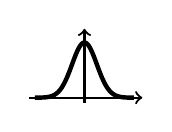
\begin{tikzpicture}
		[scale=.7]
		\draw[ultra thick, domain=-.9:.9] plot[samples=300] ({\x}, {2.7128^(-10*\x*\x)});
		\draw[->, thick] (-1.01,0)--(1.05,0);
		\draw[->, thick] (0,-.1)--(0,1.25);
	\end{tikzpicture}}
	has to do with this.
	\item How to describe and quantify mutual dependence of random events,
	and how to use such a description 
	to infer properties of ``hidden'' random events.
	\item How to apply probability theory to model real-life processes like queues
	(consisting of people or requests at an internet server).
	\item How to collaborate on solving probability problems in pairs, small groups, and online,
	and present solutions clearly and efficiently.
	\item How to design probability problems (for example, for the 
	final exam), and evaluate problems presented by others.
	\item In what ways probability theory is connected to science,
	engineering, and other branches of knowledge.
\end{enumerate}

\subsection*{Prerequisite} You should have taken at least one semester of calculus, because
the study of random variables often requires single and double integrals
and also infinite series.

\subsection*{What this course is and what it is not}

This course in probability \emph{theory} 
belongs to pure mathematics, with rigorous definitions, calculations, 
and proofs. However, the objects which we study 
are motivated by real-life applications, and so pure mathematical 
arguments often appeal to our common sense understanding of these objects. 
There will be many opportunities to explore (and discover new) connections
of the theory studied in the course with real world.

Also, this course does not discuss \emph{applications to statistics}. Probability theory focuses on 
developing mathematical side, and statistics applies these mathematical theories
to real data (coming from observations). In this course we will not discuss how to analyze data coming from observations
--- there are courses in statistics for that.

\section{Necessary information}

\subsection{Meeting times}{\ }\\

\begin{tabular}{|r|l|}
	\hline
	\textbf{Class times}  & MoWe, 2:00PM -- 3:15PM
                       \\  & Monroe Hall 124
                       \\ \hline
	\textbf{Final exam}   & Mo, May 8, 2:00PM -- 5:00PM
                       \\  & Monroe Hall 124
                       \\ \hline
\end{tabular}
\hspace{10pt}\parbox{.45\textwidth}
{

	\textbf{Instructor:} Leonid Petrov

	\textbf{Email:} We use \texttt{Slack} instead, see \Cref{comm}

	\textbf{Office:} 209 Kerchof Hall

	\textbf{Office hours:} TBA,
	% Mo 12:30PM--1:50PM and most of the weeks on We 1:00PM--1:50PM,
	or by appointment (you can make as many as you want)
}

\subsection{About the instructor}
I am an assistant professor in the Department of Mathematics at UVA, and I've
been here since 2014. My research area is probability theory (very appropriate
for this course!). More precisely, I am using exact formulas to study large
random systems. I also like computer simulations of random systems, some
examples are
\href{http://faculty.virginia.edu/petrov//blog/2016/09/16/random-heart/}{\texttt{at
this link}} or at my office door.
I'll be 
happy to tell you more if you're interested.

\subsection{Textbook}

\section{Assessing your learning}

\note{first: communicate things clearly; what probability theory is and what it is not; etc}

\subsection{Course engagement (12\%)}

There will be short quizzes, group brainstorming sessions, 
and other activities during the class
(in particular, using \texttt{Slack}),
and actively engaging in them is important to enhance 
the grasp on the foundations of probability theory and
problem-solving skills.
The grade for this part will come from: 
\begin{itemize}
	\item Quizzes.
	\item Attendance, which may sometimes be taken.
	\item Ungraded homework. All homework will be collected and some of it will be graded, see below.
	If a homework is ungraded, collecting
	it will help me identify and address 
	troubles with the material. Ungraded homework which is turned in will generally receive a ``check'' mark.
	Rarely a ``check$-$'' will be assigned if less than half of homework
	problems was attempted, or something similar.
	\item In-class work sometimes it will be collected
	and assessed, too.
	\item 
	Participation in
	polls, weekly check-ins, and
	discussions (in particular, answering other student's questions)
	in \texttt{Slack}.
\end{itemize}

\subsection{Homework (20\%)}

% engagement grade has quizzes in it; if there is no grader, then move % from HW to quizzes/engagement, easy to correct

Learning mathematics means \emph{doing} mathematics. 
In this course, this amounts to solving problems.
% (whereas at higher levels of learning math
% it would also mean proving theorems).
Homework assignments 
will help you achieve mastery of knowledge and skills pertaining to the course,
and prepare for in-class work.
You are encouraged to work together on homework assignments (also can do it online via
\texttt{Slack}, which allows private groups of up to 9 people).
Teams of two work very well. Most mathematicians work in pairs to take advantage of the challenge-defend discussions that help us understand things better.
However, each student needs to submit her/his own homework assignments,
and should work individually when writing them up to demonstrate
the understanding of the material.
The homework assignments are due approximately once a week. Some will be graded and some not ---
this will be announced in advance.

\subsection{Projects (13\%)}

There will be 2 longer projects in the course. 
The first project is a group assignment in the middle of the semester
that will help you apply your knowledge and skills
to other areas and/or to real-world situations,
and will help you enhance your collaborative and presentation skills.
You can choose to either make a computer simulation of an interesting random 
system and then experimentally describe its behavior;
or to come up with a probabilistic model of a real-world phenomenon, and 
use the model to quantitatively understand it.
Possible group projects topics are available at \url{https://TBA...}.
In the second assignment, you will get to compose a good problem for the final
exam (which even has a chance to end up in the actual exam!).
This will put you in the shoes of the instructor, and will 
let you look at the course material at a different angle.

\subsection{Tests (15\%+15\%+25\%, total: 55\%)}

There will be 2 tests during the semester, and a final exam (the second test and the exam are cumulative). 
They present an ultimate opportunity to demonstrate your knowledge and
problem-solving abilities. Tests and the exam will usually consist of problems similar to the 
ones from the textbook and lectures, and occasionally 
there can be conceptual theoretic questions.
A two-sided letter size 
formula sheet, hand-written by yourself, will be allowed on each test and the exam. 
Preparing this formula sheet will help you review the material,
and paint a systematic picture in your head.
I encourage you to collaborate on test preparation,
but needless to say that during tests and exams each student must work individually.


\section{Communication}
\label{comm}
My email is \href{mailto:petrov@virginia.edu}{petrov@virginia.edu}, 
but for the communication we will use \texttt{Slack} --- an industrial standard of work chats,
and it has a web version and apps for all platforms.
The course group is at \url{https://TBA.slack.com}, 
and you'll get an invitation to join by e-mail. 
Please let me know if you have issues with access.
It is also expected that you will bring a device with \texttt{Slack} app
(e.g., a smartphone)
to each class, 
and also check-in with me every week (by 10am on Monday).






\section{How to be successful in the course 
--- TBA}

textbook

% ``Probability'' by Jim Pitman 

% The best way to learn the subject it is to come to all classes,
% do all the homework problems and prepare for quizzes (see the schedule). Please ask me questions about things you do not understand, either in class or in my office. DON’T wait until you feel completely lost!

% Students are strongly encouraged to read the textbook. It includes many examples and extra exercises which augment the concepts discussed in the course.
% However, the textbook contains much more material than 
% will be covered in classes, so it \textbf{makes sense to come to all classes and see which parts of the textbook are actually covered}.


other references / other textbooks

khan academy, wikipedia, other places containing basic stuff on probability theory

--- office hours, availability in \texttt{Slack}, 
your fellow students, etc.

The Math Department Tutoring Center is available for helping students in this course: 
see \url{http://people.virginia.edu/~psb7p/MTCsch.html}
for more information and schedule. 

\section{Approximate course schedule}

\noindent Add/drop information: \url{http://www.virginia.edu/registrar/reginst1158.html#Deadlines}
\smallskip

\noindent \textbf{NOTE: Please don't make travel plans that conflict with tests or final exam}
\smallskip

{\setlength\LTleft{-22pt}
\setlength\LTright{-15pt}
\begin{longtable}{|L{.9cm}|L{2.5cm}|T{2.5cm}|T{2.4cm}|T{1.3cm}|T{3.5cm}|T{3.5cm}|}
\hline
\small\textbf{Week}	&\small\textbf{Topic}	&\small\textbf{Notes}	&\small\textbf{Homework}	&\small\textbf{Sections}	
&\small\textbf{Slack direct message check-in (by 10 am on Monday each week)}	&\small\textbf{Due items for the projects}	\\\hline
1:  1/18	&What is probability theory	&1/18: Introduction	&	&TBA		&	&\\\hline
2: 1/23. 1/25	&Advanced counting. Conditional probabilities	&	&	&TBA	&Individual: send me a test direct message answering why you are taking the course - to make sure it works		&\\\hline
3: 1/30. 2/1	&Repeated trials and Gaussian approximation	&2/1: group forming	&	&TBA	&Individual: briefly describe a real-world problem (preferably in one of your other courses) that you think can be accessed via probability theory	&Wed 2/1 class time: form groups of up to 6 people and let me know. It will be reflected in slack	\\\hline
4: 2/6. 2/8	&Random variables	&2/8: real-world problem discussions	&By 2/6 class time: read 
\href{https://terrytao.wordpress.com/2016/05/13/visualising-random-variables/}{\texttt{this link}} 
to see how random variables look like	&TBA	&Group: send me a test message in the private group channel to make sure it works. Also mention which real-world problem you are thinking about.	&Wed 2/8 class time: choose a real-world problem that you would like to turn into a probability problem	\\\hline
5: 2/13. 2/15	&Expectation and conditional expectation	&2/15: probability problems discussions	&	&TBA	&Group: are you doing OK with formulating your probability problem? If you are not sure talk to me during office hours - or in Slack.	&Mon 2/13 class time: Choose track: analysis or simulation. Formulate a (draft) probability problem / simulation model associated with your real-world setting	\\\hline
	&\textbf{Test 1: 2/20}	&	&	&list all sections		&	&\\\hline
6: 2/20. 2/22	&Poisson processes	&	&	&TBA	&Individual: are there any last-minute questions before the test?		&\\\hline
7: 2/27. 3/1	&Poisson processes. Exponential and gamma distributions	&3/1: project discussion before the break	&	&TBA	&Group: send me a polished version of the probability problem / simulation model you are working on	&Wed 3/1 class time: present a draft solution of your probability problem / draft simulation of your model (at least in the simplest case)	\\\hline
8: 3/13. 3/15	&Poisson processes. Exponential and gamma distributions	&	&	&TBA	&Individual: how was your break? // Group: is everything OK with the project? Need any help?	&Over the break and this week: continue working on the group project	\\\hline
9: 3/20. 3/22	&Continuous distributions. General Gaussian approximation	&3/22: full class: group presentations	&	&TBA	&Group: are you OK with your reports? who is going to present? Need any help?	&Mon 3/20 class time: group reports due; Wed 3/22: group presentations	\\\hline
10: 3/27. 3/29	&Continuous distributions	&	&	&TBA	&Individual: any feedback on the group project? Are you doing OK in the course so far?		&\\\hline
	&\textbf{Test 2: 4/3}	&	&	&list all sections		&	&\\\hline
11: 4/3. 4/5	&Joint and conditional distributions	&	&	&TBA	&Individual: are there any last-minute questions before the test?	&Sun 4/8 by 11:59pm: select topic at https://TBA on which you will compose your problem	\\\hline
12: 4/10. 4/12	&Joint and conditional distributions	&	&	&TBA	&Individual: which textbook problem did you choose? Are you doing OK with the evaluation of this textbook problem?	&Wed 4/12 class time: textbook problem evaluation due	\\\hline
13: 4/17. 4/19	&Joint and conditional distributions	&Some of the final exam review problems will be posted by 4/23	&	&TBA	&Individual: are you doing OK with composing your problem?	&Wed 4/19 class time: your problem due	\\\hline
14: 4/24. 4/26	&Bivariate normal distributions. Applications to statistics	&	&	&TBA	&Individual: are you doing OK with peer evaluation of a problem you were given?	&Sun 4/29 by 11:59pm: peer evaluation due	\\\hline
15: 5/1	&Discussion of peer evaluation and final exam review	&5/1 full class: discussion and review	&	&TBA	&Individual: which topic you found the clearest in the course? which was the muddiest?		&\\\hline
	&\textbf{Final exam: TBA}	&	&	&list all sections	&You can ask questions before the final exam in the \#general channel at any time		&\\\hline
\end{longtable}
}

\section{Policies}

\subsection{\texttt{Slack}}

Although \texttt{Slack} is a chatting app,
it should be used professionally, especially in public discussions.
The app also supports private direct messages and I encourage
to use them to collaborate on homework problems and projects, please
note that in principle the admin (i.e., myself) can obtain access to 
\textbf{all} direct messages between members of the team. The procedure would involve sending a 
paper request via the usual mail, and everyone will be notified if the direct messages are accessed ---
so this can happen only in extreme circumstances.

\subsection{Independent work, honor code}
You are required to work independently on the quizzes. So when working together with others, make sure you are preparing yourself to take the quiz independently.
The honor code is taken seriously. Any honor code violations pertaining to the quizzes will be automatically referred to the Honor Committee.

\subsection{Special needs accommodations}
All students with special needs requiring accommodations should present the appropriate paperwork from the Student Disability Access Center (SDAC). It is the student's responsibility to present this paperwork in a timely fashion and follow up with the instructor about the accommodations being offered. Accommodations for test-taking (e.g., extended time) should be arranged at least 5 business days before an exam.

% \newpage
%
% \begin{center}
%   {\large\textbf{Plan for the first class}}
% \end{center}
%
% \note{see slack and notes in evernote}
%
% Go over policies, also about slack.
%
%
% \newpage
%
% \begin{center}
%   \hfill date
%   \\
%   {\large\textbf{Project 1: Group assignment}}
%   \\
%   \texttt{due dates: TBA by TBA, TBA by TBA, TBA by TBA}
% \end{center}
%
% \medskip
%
% The purpose of this project is to put you in a collaborative environment,
% and help you explore how probability theory can be applied
% to real-world situations.
% In fact, nowadays applications of probability theory (along with statistics,
% and sometimes under the names of modeling or operations research)
% span almost every area of human knowledge and activity, so there is a lot to choose from.
%
% There are two tracks to choose for this assignment: \emph{analysis} or \emph{simulation}.
% The analysis track is suitable for anyone in the course, while
% your group should choose the simulation track only if you
% are comfortable with computer programming
% and are able to code stochastic simulations (specific programming language does not matter).
%
% There are following general steps to this project:
% \begin{enumerate}[\bf{}1.]
%   \item Form groups of up to 6 students by TBA, and let me know.
%   I will organize private group channels in \texttt{Slack} in which you can communicate.
%   and I will also be present there to help you at any time.
%   (Note: you can also create a private direct message group
%   to discuss the problem completely on your own.)
%   \item Choose a real-world situation or problem that you would like to
%   translate into probabilistic language. This can be related
%   to some topic from your other course, or a problem you care about --- so anything you find interesting
%   (well, you should at least feel that some probabilistic approach could be applied here).
%   Do this step in your group by TBA, and let me know. We will briefly discuss
%   problems you choose in class on TBA.
%   \item In the next step, by TBA, you need to choose a track (analysis or simulation)
%   and formulate a probabilistic system (in mathematical language)
%   related to your real-world problem. In this step you will inevitably
%   oversimplify the real-world situation, and this is fine --- because we want
%   mathematics to say at least something about your problem.
%   (Note: you can always complicate things
%   afterwards a little, don't worry about oversimplifying in the beginning.)
%   In this step communication with me is very important, since I have a good idea
%   which problems are approachable with tools we are learning in this course.
%   \item The next step (by TBA) depends on your track:
%   \begin{itemize}
%     \item In the analysis track, you should present a solution to the probability problem you formulated,
%     at least in the very simple case.
%     This solution can use any computer algebra system, etc., so that
%     you are not restricted only to problems you can solve by hand.
%
%     \item In the simulation track, you will build a computer simulation
%     of your situation. This track could in principle allow you to
%     take a more complicated model
%     than the analysis track, but this will then require simulating it in detail.
%   \end{itemize}
%   This step will lead to a report,
%   first draft of which is due by TBA,
%   and the
%   final version due by TBA.
%   The work on the analysis or simulation should tap back into the real-world problem,
%   and your work here should lead to you being able to say at least something about the real-world model
%   you started from.
%   \item Moreover, on TBA we will have presentations in which one member of each group
%   will have 10 minutes to briefly explain the project and conclusions.
% \end{enumerate}
%
% \razdel{Criteria}
%
% Participation in this project and timely submitting your work is very important.
% The most important part of the project in terms of grading is to get your math
% right --- to accurately formulate the problem or the system you're going to simulate,
% and present correct and accurate reasoning and discussion.
% It is also important that you understand and articulate in which aspects you are oversimplifying
% the real-world problem to get a mathematically tangible model.
% Because you are only beginning to learn probability theory
% and because the time is limited, your models inevitably will lack some (or even most) of the
% properties of a real-world problem --- and this is fine, as long as
% you understand where your simplifications were performed.
% If research and obtain
% any outside numerical/qualitative data to input into your models,
% please cite the source (any format)
% to explain where this input comes from.
%
% Since the presentation part of the project falls on the shoulders of one member of each
% group, this activity counts as for training purposes only.
%
% I expect that most groups will get a full grade on this assignment,
% and stellar work will also receive bonus points.
%
% \razdel{Analysis example}
%
% Let me give you one good example of a real-world problem which can be turned into a
% probability problem (this is more for the analysis track).
% As we know, the airlines sell more tickets to a flight than there are
% seats on it. This is because some passengers do not show up for the flight,
% and so company gets free money. But if in fact more passengers show up for the flight,
% then the company has to pay some of them to not fly, and rebook them to different flights,
% or maybe even pay for the hotel --- so this costs something.
% This leads to a simple probability problem:
% \begin{quote}
%   Assume that there are 300 seats on the plane,
%   and the company sells 320 tickets. Let each person
%   independently decide to show or to not show to the flight
%   with probability $0.95$ (i.e., with probability $0.05$ the person does not show up).
%   What is the (approximate) probability that the flight is overbooked?
% \end{quote}
% The solution of this problem is the following:
% \begin{quote}
%   The number of people
%   showing up for the flight is equal to $S_{320}$, the binomial
%   random variable corresponding to 320 coin tosses, with probability
%   of success $p=0.95$. The mean is $320\cdot p=304$, and the standard deviation
%   is $\sqrt{320\cdot p(1-p)}=3.9$.
%   We see that by the Gaussian approximation (the part ``$+\frac12$'' is the correction):
%   \begin{equation*}
%     P(S_{320}>300)=P\left(\frac{S_{320}-304}{3.9}>\frac{300+\frac12-304}{3.9}\right)\approx
%     P(Z>-0.897436)\approx 0.82.
%   \end{equation*}
%   That is, the flight is overbooked with probability $0.82$.
%   This means that the airline is probably selling to many
%   tickets, and to avoid overbooking with this high probability it maybe should
%   sell less of them.
% \end{quote}
% In formulating this problem, we made the following assumptions/simplifications:
% \begin{itemize}
%   \item The airline company has to decide in advance
%   how many tickets it would sell, while in reality this decision can be made
%   while the ticket sale is still ongoing.
%   \item Each passenger is independent in his/her decision to fly or not to fly.
%   This is unrealistic because many passengers travel in families.
%   \item The exact parameters $p=0.95$ and that the airline sells $320$
%   tickets are completely arbitrary, and it would be nice to find some actual numbers
%   if possible (especially for $p$).
%   \item The Gaussian approximation is quite accurate for the binomial
%   random variable in the problem, but using a computer algebra system
%   you can actually compute the exact probability
%   of overbooking --- it is $0.817679$, which is indeed very close.
% \end{itemize}
%
% The example above (problem, solution, discussion of assumptions/simplifications,
% plus a
% discussion of how the probability
% problem allows to infer something about the
% real-world problem we started with)
% is good as a first draft of a successful project.
% That is, a first attempt is to just consider a very simple situation,
% and be able to say at least something.
%
% A successful project growing out of this example
% should also contain the following:
% \begin{itemize}
%   \item A quick research (start with googling) on what is the actual probability $p$ is.
%   (As with any outside data, please cite the source if you are using this data.)
%   \item Discussion/modifications for the cases when the decisions
%   made by passengers to not show are not independent --- i.e.,
%   a typical flight contains of some number of individual travelers, some number of
%   pair travelers, etc.; a quick research of how a realistic distribution
%   of passenger groups looks like would be nice.
%   \item Added cost factors and cost analysis. This should start with a quick research
%   on how much more it costs airlines to handle overbooked passengers vs.
%   average ticket cost (in fact, ticket costs also rise
%   closer to the date of the flight, and this is another aspect that could be considered).
%   Then in the analysis above you can find optimal (from the cost perspective)
%   number of tickets to sell to a 300-seat flight.
%   This part exactly corresponds to a probability analysis being able to
%   say something about the real-world problem.
% \end{itemize}
% We see that there are many directions
% into which this could
% grow (and many more not mentioned above!), but accurately considering all the above additional points,
% and complementing an exploration of
% some of these directions
% with correct math would count as a
% successful project.
%
% \razdel{Simulation example}
%
% TBA
%
% \newpage
%
% \begin{center}
%   \hfill date
%   \\
%   {\large\textbf{Project 2: Final exam problem}}
%   \\
%   \texttt{due dates: TBA by TBA, TBA by TBA, TBA by TBA}
% \end{center}
%
% \medskip
%
% After most of the course is over, it is time for me to
% compose the final exam --- with your help.
% I invite you to reflect on topics discussed and skills developed this semester,
% and compose one problem for the final exam. The problems you come up with
% will be added to the list of review problems,
% and some will actually end up as a part of the final exam.
%
% \razdel{Part 1. Deep solution and evaluation of a textbook problem}
%
% To be able to design your own problem, first
% analyze an existing one.
% \textbf{Pick a problem} from the textbook which you didn't see before
% (you may even pick a problem at random until you encounter one you never saw).
% Read the questions below. Then,
% using the tools you learned during lectures and
% from the textbook, \textbf{solve this problem and get an answer}.
% If needed, you can consult any other sources
% or your fellow students,
% use calculator/computer (no matter how advanced) ---
% to make sure you got the solution and the answer right.
%
% Briefly respond to the following questions (please read them before solving!):
%
% \begin{enumerate}[\bf{}1.]
%   \item What knowledge and skills/tools did you need to solve this problem?
%   \item Are there any nontrivial observations/ideas needed to solve the problem? Is it too hard? Too easy?
%   \item (if applicable) Is the answer given in the textbook correct? Is it complete? Is it clearly understandable? Was it hard to compare your answer with the textbook's one (even if
%   you got a correct answer, it could be in a different form)?
%   \item Are there common-sense mechanisms which can help ``debug'' your answer?
%   (like: ``if the problem asks for a probability, it must be between 0 and 1'')
%   \item Out of 45 students in our class, how many do you think will solve the problem and get the right answer if it is given as a part of the final
%   exam?
%   \item Is the problem applicable to real life/other branches of knowledge? How/why not?\\
%   (\emph{optional}) Could you imagine a real-world situation in which a similar problem can be applicable?
%   \item (\emph{optional})
%   Time
%   how long it took to write a draft of the solution
%   and get an answer, and share this information with me.
% \end{enumerate}
%
% \textbf{Submit the problem, a write-up of its solution, and brief answers to the above questions on Collab by TBA}.
%
% \emph{Criteria}:
% Make sure to present a correct and complete solution.
% Your write-up of a solution
% must be clear and concise. If you use a random variable or event not given
% in the statement of the problem, you must first define that random variable or event.
% If you have to say something that is not a mathematical expression, say it in complete English sentences.
% Most successful write ups will take some time to get on the page.
% The work in this part will receive one of the two marks:
% ``poor/no work'' and ``good''.
%
% \razdel{Part 2. Designing your own problem}
%
% Think about the problem you solved in part 1 --- should this or a similar
% problem appear on the final exam? Or would you modify it in some way?
% Think about the topics in the course, and pick the one you like most.
% \textbf{Sign up} for this topic at
% \url{https://TBA} by TBA (first come, first serve).
% Then \textbf{compose a good problem on this topic}.
%
% Aim for a medium-level problem (not too easy, not too hard).
% Try to invent a more realistic problem, which is somewhat related to
% other areas of science or to a real-world situation.
%
% \emph{Note}: If you choose to make your problem similar to one of the textbook
% or homework/quiz problems, try to make the context of the problem
% closer to a real-world situation. That is, imagine a situation in the real life
% when a similar problem might arise, and use it as a setup.
%
% \textbf{Submit your problem, its brief solution and answer on Collab by TBA}.
%
% The solution your present in part 2 does not have to be as clear and
% detailed as in part 1, just make sure it is understandable
% and the answer is correct.
%
% \emph{Criteria}:
% The problem you submit will receive one of the three marks:
% ``poor/no work'', ``good'', and ``great''.
% To avoid getting a ``poor'' mark,
% the language of the problem should be clear, concise, and unambiguous.
% Make sure that there is no way that some of students in our class
% can read the problem wrong (you can seek quick feedback from other students on that
% while you're working on your problem).
% An advantage is if the problem describes a real-world situation.
% Too easy or unnecessarily hard
% problems will not be ranked ``great''.
% Make sure to present a correct and complete solution to the problem.
%
% \razdel{Part 3. Peer evaluation}
%
% You will receive a problem composed by another student, together with the answer.
% \textbf{Solve the problem, write its solution in detail similarly to part 1,
% and answer the questions as in part 1}. Same criteria as in part 1 will be applied.
%
% \textbf{Submit this work on Collab by TBA}. Note that your feedback can and likely will be shared
% with the author of the problem.
% \textbf{On 5/1 in our last class we will have a discussion
% wrapping up the project, which will also be a
% review session for the final exam}.
%
% % I won't give preferences to problems I choose, just mention (after the exam). This is because I have to
% % balance the exam, and there are much less problems in the exam than what I'll receive.




\end{document}
